\chapter{Vocal Accommodation in Real-World Sales Calls}
\label{chap:conv_analysis}

\lettrine{V}{ocal} accommodation occurs in spontaneous \acl{hhi}.
Its effects are investigated in this chapter using a collection of authentic sales calls.
As speaking is an essential part of sales representatives' everyday work, controlling their it is key for their deals' success.
In addition to the extent of the effects, it is also examined which speaker initiated them.

\pagebreak

\acresetall

\section{Harnessing speech alignment for conversation intelligence}
\label{sec:conversation_intelligence}

Sales leaders have always been impelled to be able to reason why some of their representatives (henceforth \emph{reps} or \emph{\acp{ae}}) consistently attain and even exceed their goals while others do not \citep{Kovac2017its}.
Yet, sales executives rely on data that is inherently flawed, as it is based on reports from sources like \ac{crm} systems.
Such systems only contain \enquote{dry} details about deals' stage, along with high-level numeric data and some, typically subjective, estimations regarding their potential in the following stages.
That leaves the executives in the dark regarding the happenings at the front lines and the small-scale, day-to-day conducts and modi operandi, which are critical for the \acp{ae}' success.
As a result, the reasons for losing or winning a deal often remain a riddle, making sales seem like art based on anecdotes rather than a scientifically explainable practice \citep{Yohn2016best, Martin2017six}.
In his seminal book, \citet{Gladwell2006tipping} states that \textquote[p.\ 83]{Part of what it means to have a persuasive personality is that you can draw others into your own rhythms and dictate the terms of the interaction}.
Supporting that, \citet{Orlob2018nine} found that star reps\footnote{Sales representative whose performances (and specifically their closed-deals rate) are exceptionally high are often referred to as \emph{star reps}.
The specific criteria typically include a wide range of behavioral and business metrics, but those are defined internally per company and do not have a common absolute definition.} are able to make prospects increase their speaking rate to match theirs, bringing the two sides closer with respect to this speech property.
However, the scientific analysis is far from their everyday work, and such phenomena are passed on as general tips and are not taught or explained in detail to the \acp{ae}.
\Ac{c-iq} systems aim to bridge over this gap and connect the scientific side of sales to the field to help reps to improve their performance using measured, interpretable methods.
Being part of verbal interaction, vocal accommodation is a facet that can shed light on certain processes occurring during a sales call.
Indeed, this phenomenon has been given attention in analyses and evaluations of \acp{ae}.
It was found, for example, that distinguished sales reps let the prospects talk more and keep certain parts of the calls shorter than low-performing reps \citep{Orlob2017winning}.

\Acf{f0} can be interpreted and explained by people with no phonetic training, like \acp{ae}.
Furthermore, speakers can easily control it, making it a tangible tool for the \acp{ae} to exploit in their sales calls.
This, as opposed to more complex acoustic features like \acp{mfcc} or changes in the \ac{ltas} that are often used in phonetic accommodation studies \citep[e.g.,][]{Levitan2011measuring, Borrie2019syncing} and are hard to directly control during a conversation.
For this reason, the analysis presented in this chapter focus on \ac{f0}, although other suprasegmental features showed similar effects.
For this, a large-scale corpus of real-world sales conversations was collected (\cref{sec:dataset_calls}).
Beside the size advantage, the use of such a corpus takes the study of vocal accommodation out from the controlled laboratory environment into the wild for a practical goal.
The conversations in this corpus are therefore highly flexible and generally structure-free, unlike lab experiments like those presented in \cref{chap:shadowing_in_sung_music_and_human_computer_interaction}.
It is also important to note that beside the overall goal of closing a good deal, there are no specific instructions given to the speakers on both sides regarding how to speak or what to say.
By extension, they are also more authentic and spontaneous, since the interlocutors are driven solely by their own behavior and motivation to succeed and are not given an artificial temporary role.
\Ac{crqa} \citep{Zbilut1998detecting}, a bivariate correlation technique, was used for the analysis (\cref{sec:crqa}).
This method finds instances where coordinates of two time series occur close to each other within a certain radius in a phase-space continuum.
Since \ac{crqa} evaluates the degree to which the similarity of two time series changes over time and can also determine the leading relationship between them, it is suitable and informative for analyzing accommodation.
The contributions of this study are therefore both in the methodology for measuring accommodation and its practical application in a real-world scenario.

\subsection{\Acl{c-iq}}
\label{subsec:conversation_intelligence}

The way people communicate and behave in inter-person situation influences the manner in which conversations unfold.
These influences can be analyzed and interpreted to uncover conversation-level trends, which may differ from the linear turn-by-turn changes.
\Acf{c-iq} is a relatively newly coined term and a field of research that flourished due to advancements in neuroscience, communication science, and \acl{ml}.
It complements other types of human intelligence, like \emph{emotional intelligence} \citep[c.f.\ \emph{Theory of Multiple Intelligences}][]{Gardner1983frames, Davis2011theory}, as the ensemble of conversational aspects in human communication \emph{beyond the surface words and shared information}.
\citet{Glaser2016conversational} explains and demonstrates how \ac{c-iq} can be learned and improved, with emphasis on the ability to gain trust and maintain more successful communication.
Although \ac{c-iq} comprises many further aspects that are beyond the scope of this work, the overarching idea that improving communication quality is a skill that can be learned is highly relevant for vocal accommodation but has not been explored in previous work.

Narrowing down this broad idea, \citet{SilberVarod2018human} discusses how conversations can be \emph{managed}.
This includes both the structure and evolution of a conversation over time and the dynamics between the interlocutors' based on their roles in it.
Noticeably, it is concluded that some speech-related phenomena in conversations tend to be more complex and unpredictable than they seem in their surface form.
One of those phenomena is phonetic entrainment, which was found in long-term influences of the speakers on each other.
Such works dealing with managing spoken interactions become even more relevant with the growing interest in intelligent conversational systems for personal usage \citep{Mehr2017artificial}.
Recently, the importance of \ac{c-iq} has pervaded the enterprise sector and created new businesses.
Two main motivations were the utilization of computer-based customer services \citep{Gnewuch2017towards} and the use of conversation intelligence services for inside sales calls to train \acp{ae} and improve their performance \citep{Orlob2017winning, Orlob2017separates}.

\subsection{Inside sales}
\label{subsec:inside_sales}

In recent years, many companies have adopted the concept of \emph{inside sales}, where \ac{b2b} sales are done using web-based conferencing solutions, as opposed to face-to-face meetings with the clients.
Recent technological advancements allow automatic recording and transcription of those inside sales calls and aggregation of large-scale datasets.
These datasets include the audio of the calls and sometimes annotations such as the speaker turns and performance rating of the \ac{ae}.
These conversations have a typical process:
First, a \ac{sdr} reaches out to a potential client (the \emph{prospect}) who has expressed interest in the company's product, which initiates a \emph{lead}.
Subsequently, the \ac{sdr} shares basic details about the product and how it can help the prospect.
Finally, if the \ac{sdr} has managed to elicit initial interest, the lead turns into an \emph{opportunity}, and a demo call with a sales representative is scheduled.
Such demo calls are often done using a web conferencing tool, such as Zoom\footnote{\url{https://zoom.us}} or GoToMeeting\footnote{\url{https://www.gotomeeting.com}}, which allows both sides to share their webcams and screens.
A collection of such initial opportunity calls is analyzed in here (\cref{sec:dataset_calls}).
It is known in the \ac{b2b} industry that since these calls are the first personal contact, the behavior and verbal skills of the \ac{ae} have a large weight in the success of the call.

\subsection{Influence of speaker roles}
\label{subsec:speaker_roles_and_influences}

Although accommodation is not a traditional measure in \ac{c-iq}, there have been attempts to use it as an additional factor for evaluating conversations.
\citet{Glaser2016conversational} emphasizes the importance of the turn-level alignment between speakers in a business call.
Lack of alignment may result in a skeptic and even resisting behavior that might lower the success chances of the call \citep[see also Table 2 in][]{Glaser2014conversational}.
At the very least, this demonstrates effect of interlocutors being attentive not only to the content of the conversation, but also to the way it is delivered.
In \ac{b2b} calls, this is especially relevant for the \acp{ae}.
\citet{SilberVarod2018human} shows how convergence effects indicate power relations facets of \ac{c-iq} analyses.
Specifically, speaker \enquote{dominancy} is often hard to spot on the surface, but becomes more prominent when examining the vocal relations between the speakers.
Furthermore, \citet{Abrego2011effects} discuss how the judgment of a speaker's role in a conversation influences the phonetic productions and vice versa.
Analyses like these improve the understanding of vocal behaviors in \ac{hhi}.
The idea of speakers' behavior being modified due to their role in the conversation and their perception of the other interlocutor is a key concept for the presented study.

\section{Dataset and feature extraction}
\label{sec:dataset_calls}

A collection of real-world calls with similar characteristics to those described in \cref{subsec:inside_sales} was used in the study presented here.
These calls were all made by trained sales representatives and were aimed at high-stakes deals\footnote{In this case, around US\$\num100,000 each, as opposed to occasional mass calls to random people for selling small products where the deals are very small in comparison.
The reps know that their performances are evaluated, pushing them to do their best in every single call.}.
To make the collection more homogeneous, calls of a single sales company were selected.
Another constraint was that the collection comprised only calls from a very early stage of the sales opportunity (see \cref{subsec:inside_sales}) that is also the first encounter between the participating \ac{ae} and the prospect.
Therefore, the observed behavior patterns in these conversation are not influenced by the previous verbal interactions between the two speakers.
the structure of these calls typically includes an overview of the prospect's business, followed by a deeper explanation of the sold product by the salesperson, and typically further negotiations.
It is important to note that although professional \acp{ae} prepare for these calls as part of the daily work, they are still spontaneous and are in no way scripted.
The calls in this collection were conducted using the Zoom video conferencing platform and were recorded automatically -- without any intervention from either side -- by an external conversation intelligence service.
% Gong.io's system, which provides conversation intelligence services to said company.
The calls were transcribed and diarized using the internal \ac{asr} system of the service.
Participants were notified of the recording, in compliance with all relevant laws and rights.

In total, 708 calls were analyzed, spanning more than \SI{442}{hours} (mean 37.5 $\pm$15 minutes).
Furthermore, only calls longer than 15 minutes were selected, as shorter calls are often unsuccessful connection attempts or brief updates that are not representative of the desired conversation structure and dynamics.
A single \ac{ae} and a single prospect participated in each call.
Call recording started immediately following the first greet from the prospect's side, and stopped when the \ac{ae} terminated it.
This eliminates segments during which one party is waiting for the other to join, and keeps only segments where both parties are present.
%The 26 \acp{ae} (12 female) in these calls formed 87 unique interlocutor pairs with different prospects.
Each prospect only ever spoke with one of the 26 \acp{ae} (12 female).
Both interlocutors in all the conversation were native speakers of American English and worked in an English-speaking company.
For the purpose of this study, a call was defined as successful if a follow-up call under a more advanced stage was initiated or when an advancement in the opportunity was marked within one month.
These criteria follow common conventions of measuring success of \ac{b2b} calls\footnote{The benchmarks for successful deals are much more elaborate in practice and usually consider an entire selling process that comprises a series of calls.
However, many of those criteria are not relevant or cannot be enforced in the scope of this study.}.
This resulted in 51 calls (\SI{7.2}{\percent}) being defined as successful, which is within the industry-standard ratio for such early-stage calls.
%Failed calls lasted 37~$\pm$15 minutes on average and successful calls 42~$\pm$16.5 minutes.
%A two-sample Wilcoxon test \citep{Wilcoxon1945individual} between failed and successful call durations yielded a p-value of 0.04 with a confidence level of \SI{95}{\percent}, confirming their differentiable distributions.
%It goes without saying that the labels of both criteria are noisy, as sales opportunities might be lost due to various other factors.
%To minimize such cases, calls done by personnel that are not sales people in the customer companies were filtered out.
%Following that, we hypothesized that successful sales calls would show more distinct speech patterns and vocal accommodation behaviors than unsuccessful calls.

To increase temporal resolution, the audio signals were split into two-second slices (cf.\ \cref{sec:analysis_hhci}).
This increases the number of datapoints the \ac{crqa} considers.
Splitting the turns also creates equal, consecutive, and more comparable time units in the conversations without introducing artificial boundaries by dividing it into a pre-defined number of parts based on some arbitrary criterion.
The slicing was done per turn, so that a slice contains only the speech of a single speaker.
Any remainder of a turn got a slice of its own.
When a speaker was not speaking (e.g., during the turn of the other interlocutor), it was assumed that the last produced value was maintained until the speech is renewed and a new value can be measured.
This way, no discontinuities are created and the same number of datapoints can be extracted for both speakers to create a better temporal representation of the conversation.
Feature extraction was done using the system described in \cref{chap:web-based_responsive_spoken_dialogue_system} \citep[and see][]{Raveh2018Specom}.
The values were measured using Praat \citep{Boersma2018praat} scripts that extracted the \ac{f0} value from the middle of each slice.
Afterward, the list of measures was turned into two equally long time series:
First, the values for each speaker were separated into two lists.
Subsequently, missing values, e.g., due to non-speech slice, were replaced by the most recent valid value of their respective speaker, as motivated above.
Finally, if there were missing values at the beginning of a list, the first valid value of that list was used, under the assumption that the first utterance represents the immediate time prior to it.
The resulting two lists had the same number of values representing the same timestamps along a single conversation, and were used as the input time series for the \ac{crqa}, which can be assumed to be non-seasonal and non-stationary.
This process was performed independently for each conversation.

\section[\Acl{crqa}]{\Acl{crqa} for measuring vocal accommodation in conversations}
\label{sec:crqa}

\subsection{Capturing accommodation with \acs{crqa}}
\label{subsec:capturing_behaviors}

Depending on the circumstances, \ac{hhi} may involve different communication channels, such as facial expression, hand gestures, and eye gaze.
The analyses here concentrate on the phonetic level, as it is the primary modality used for conveying information in sales calls, even when video or screen sharing functionalities are available as well.
It has been shown in studies based on \ac{cat} (\cref{sec:communication_accommodation_theory}) that
mutual vocal adjustments in \ac{hhi} increase the success rates of conversations \citep{Pickering2004behavioral} and affects the social distance between speakers \citep{Schweitzer2017social}.
Accordingly, effects of the same nature have been found in \ac{b2b} sales calls as well \citep{Orlob2018roi}.

Linear methods for measuring accommodation rely on the chronological, turn-by-turn order of the interaction.
As discussed in \Cref{subsec:limitations_of_did,fig:accommodation_types}, these methods are limited to the detection of local effects that evolve gradually across adjacent turns.
Non-linear methods, on the other hand, do not rely on turn adjacency and can find long-term relations between the speakers' speech productions on the conversation level.
For instance, accommodation may occurred at some point in the beginning and be continued at a later time.
This is especially useful for long interaction, like the sales calls in the corpus used here, where the insights from more general view are useful for improving performance.
This encourages treating the interactions as continuous event rather discrete parts, and opens a variety of time series analysis methods.
\Ac{crqa} is one such method, which offers more than the direct comparison of large pre-defined chunks of neighboring turns, as is typically done in accommodation studies in spontaneous conversations \citep[e.g.,][]{Levitan2013entrainment, Rahimi2018weighting}.
It utilizes phase-space embedding, which describes the temporal evolution of trajectories of a dynamic system by projecting their embedding onto some common space.

An overview of \ac{crqa}is given by \citet{Wallot2018analyzing}.
At its core, this method compares delayed instances of the phase-space trajectories of two time series.
This allows for finding more general patterns in the time series characteristics and how they interact.
It is especially suitable for studying accommodation and related phenomena, as it detects times in which the time series (here, the speakers' productions) are similar.
Moreover, it can mathematically show which of the time series lead the alignments or whether the changes were done in synchrony.
This is useful for describing different the types of accommodation described in \cref{subsec:variation_types}, like synchrony and alignment.
\Ac{crqa} has already been used in \ac{hhi} research.
For instance, \citet{Duran2017conversing} used it for analyzing and predicting speech differences in scenarios with disagreement and deception tasks.
A similar method was used by \citep{Borrie2019syncing} to measure conversational entrainment for assessing speech pathology.
It was found that sessions with longer periods of synchronization were rated as more successful by therapists.
This is a good example of a cooperative interaction with a common goal that accommodation contributes to its success.
In sum, \ac{crqa} can be used to objectively quantify and describe accommodation between speakers dynamically across entire conversations.
\Cref{subsec:recurrence_detection,subsec:parameters_crqa} explain the technicalities of \ac{crqa}, how its output can be interpreted, and how it is used in the study presented in this chapter.
%
\begin{figure}
	\centering
	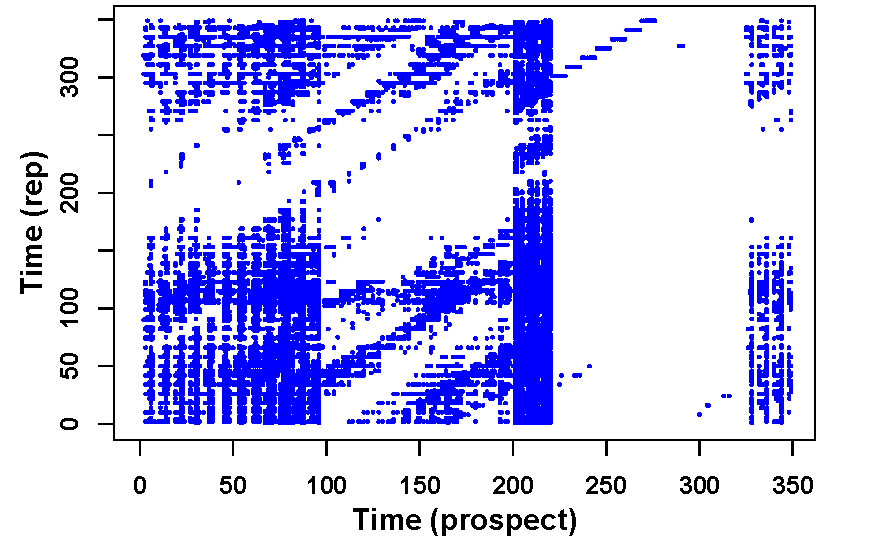
\includegraphics[width=\linewidth]{crqa_plot_115993376241473405}
	\caption[\acs{crqa} analysis of pitch in a sales call]
		{A recurrence plot generated for one of the analyzed conversations.
		The y-axis marks the conversation timeline, in slices, of the \ac{ae}, and the x-axis of the prospect.
		Each blue dot represents a co-visitation of a similar state.
		Blue dots forming a diagonal line indicate sustained recurrence between the two speakers (see description of NRLINE in \cref{subsec:output_values} for details).
		Note that the timestamps on the axes are not the slices, but the embedded call time.
		For example, the diagonal structures between timestamps 100 and 200 of the x-axis show such lasting recurrence.
		Diagonal lines above the \acl{los} (\acs{los}; the central diagonal line) indicate that the speaker on the y-axis leads the x-axis, and vice versa for lines below the \ac{los}.
		The blank area between timestamps 220 and 330 of the x-axis point to a portion of the call where the speakers were more distant from each other.}
	\label{fig:crqa_plot}
\end{figure}

\subsection{Recurrence detection}
\label{subsec:recurrence_detection}

\Ac{rqa} is a method for non-linear data analysis that quantifies the number and duration of recurrences within a dynamical system presented by its state-space trajectory, which is typically the realization of a sampled time series.
It was introduced by \citet{Zbilut1992embeddings} and later extended by \citet{Webber2005recurrence, Marwan2002cross}.
A \emph{recurrence} (also, \emph{re-visitation}) is a time in which the trajectory returns to a state it has visited before.
Recurrence can, therefore, be defined as the binary function
%
\begin{equation}
	\label{eq:recurrence}
	R_{i,j} =
	\begin{cases}
		1,	&	\text{if} \quad \lVert \vec{x}(i)-\vec{x}(j) \rVert_d \leq \varepsilon \\
		0,	&	\text{otherwise} \\
	\end{cases},
\end{equation}
%
where $i$ and $j$ are samples of the time series, $d$ is the number of embedding dimensions, and $\varepsilon$ is the threshold radius distance below which two cross-trajectory points are considered similar, as explained in \cref{subsec:parameters_crqa}.
\Ac{crqa} is an extension of \ac{rqa} for analyzing recurrence quantification between \emph{two different} time series rather than a single one.
As such, \ac{crqa} is a quantification technique for non-linear data analysis that describes when and to what extent concurrences (or \emph{co-visitations}) occur in the two time series.
These quantification techniques are based on \emph{recurrence plots} that for each pair of samples $i$ and $j$ from the two time series show the times at which a phase space trajectory is similar, i.e., when $TS_i \approx TS_j$ (and see \cref{fig:crqa_plot}).
The recurrent points $R_{i,j}$ are colored if their value is 1 or remain unmarked otherwise.
The main diagonal of the plot is called the \acf{los}.
A high number of recurrences along this line indicates synchrony between the time series.
However, diagonal recurrence lines can be formed above and below the \ac{los}.
Such diagonals, especially longer ones, represent delayed (lagged) synchrony between the time series and can be used as an assessment of similarity between the processes.
In the context of accommodation, these diagonals imply accommodative processes led by one of the interlocutors.
If the diagonal stretches above the \ac{los}, the speaker plotted on the x-axis leads the accommodation and vice versa.
The closer the diagonal is from the \ac{los}, the faster the process occurred, i.e., the led speaker aligned his behavior to the leading speaker after a shorter time.
This ability to not only detect latent accommodation but also determine its initiator on a fine-grained time scale enables the description and detection of more complex accommodation behavior, such as delayed synchrony (\cref{fig:accommodation_types}).

\subsection{Parameter tuning}
\label{subsec:parameters_crqa}

\Ac{crqa} has three parameters:

\begin{enumerate}
	\item \textbf{Delay} -- estimates the temporal shift required to make the two time series maximally correlated.
	It is measured by the same time unit as the time series (here, two-second slices; see \cref{sec:dataset_calls}).
	
	\item \textbf{Embedding dimensions} -- are the number of dimensions into which the datapoints are embedded.
	These dimensions are delayed copies of the original time series $TS_t$ created by adding a lag $k$ to them.
	Typically, multiple $n$ lags are considered, which create the dimensions of embedding $TS_{t + nk}$.
	
	\item \textbf{Radius} -- determines the margin within which two datapoints constitute a recurrent instance.
	Distances between the datapoints are measured in the embedded space defined by embedding dimensions, using the same unit used for measuring the values of the time series.
\end{enumerate}
%
\begin{figure}
	\centering
	\begin{minipage}{.45\linewidth}
		\centering
		\includegraphics[width=\linewidth]{ami}
		\caption[Average mutual information of time series as function of lag]
			{The average mutual information of the time series values as a function of the lags considered.
			The x-axis shows the considered lags and the y-axis the mutual information index (AMI) in bits.}
		\label{fig:ami}
	\end{minipage}%
	\hfill
	\begin{minipage}{.45\linewidth}
		\centering
		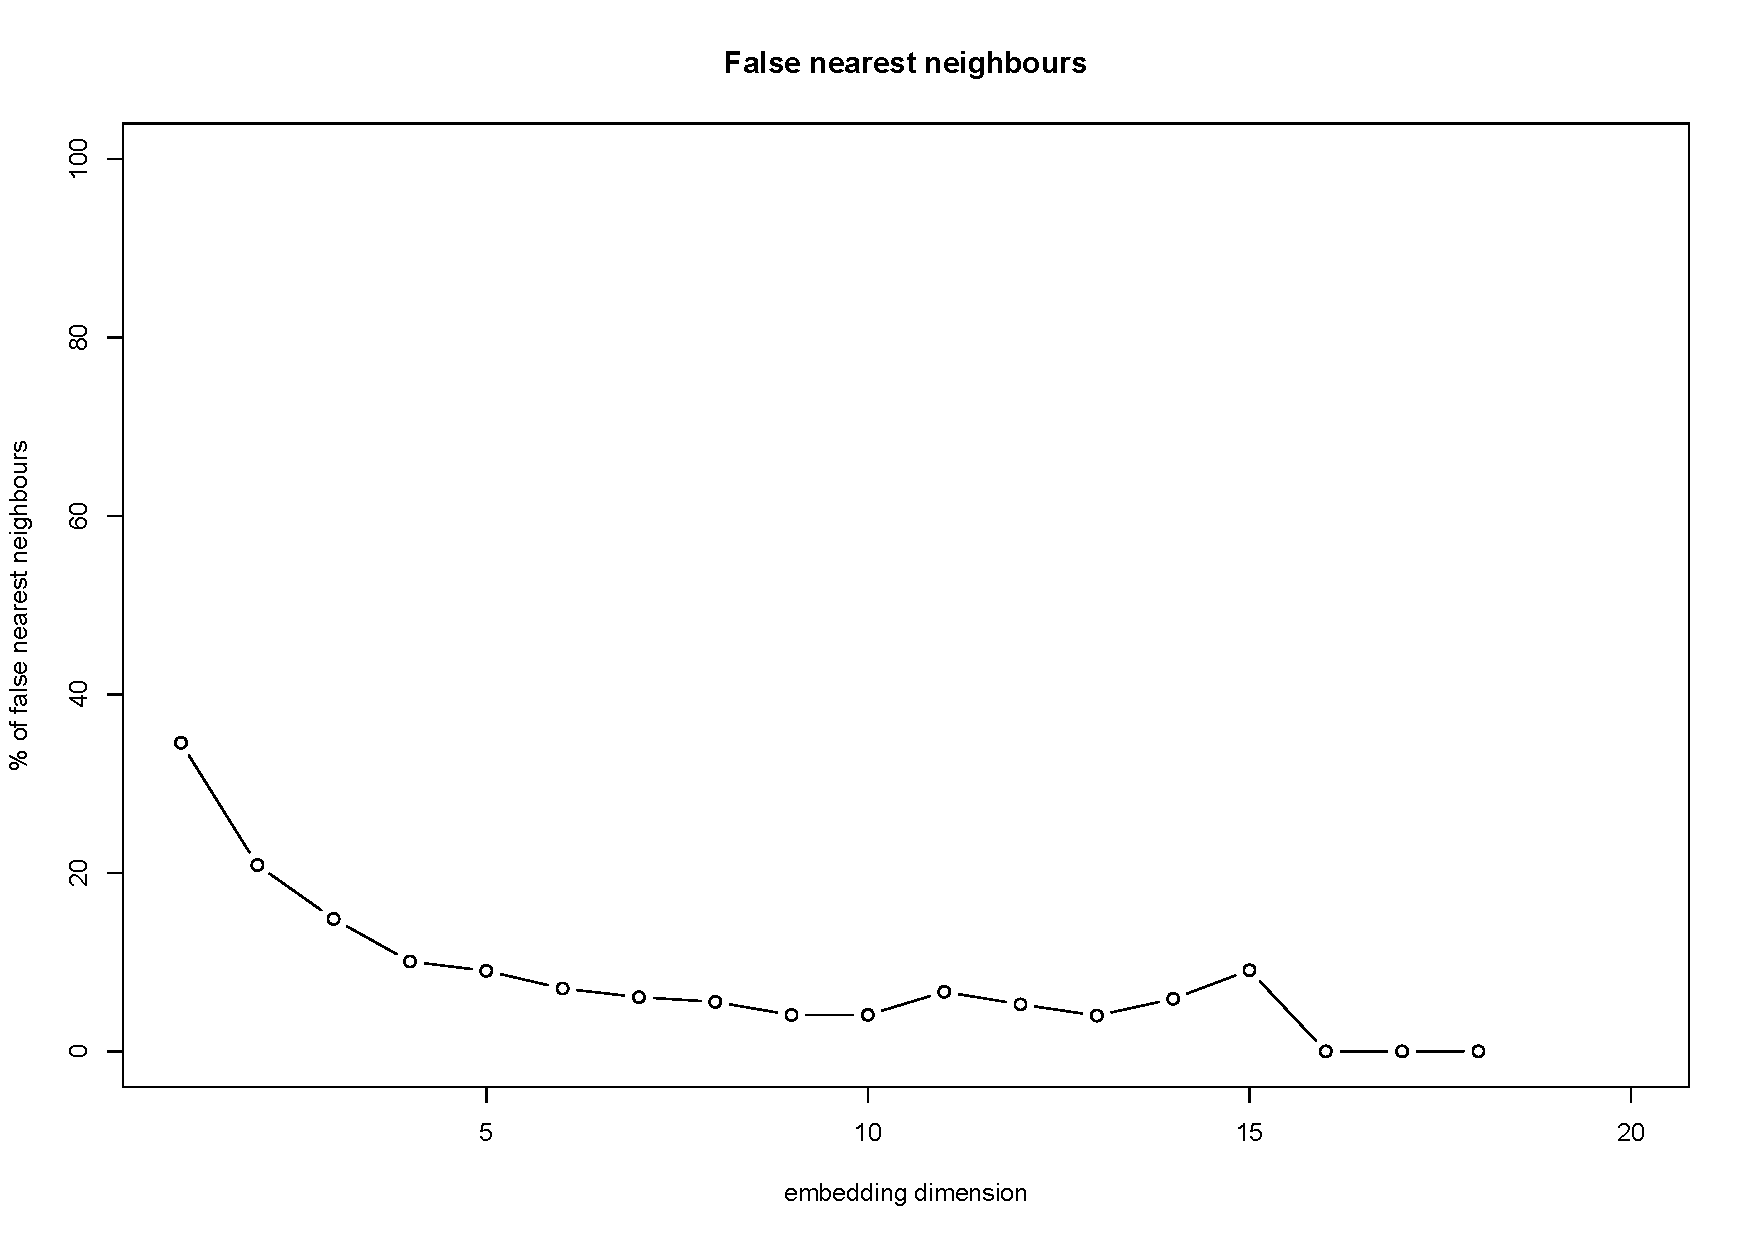
\includegraphics[width=\linewidth]{false_NN}
		\caption[Embedded dimensions optimization]
			{False nearest neighbors percentage as a function of the number of embedded dimensions.
			The x-axis show the considered numbers of embedded dimensions and the y-axis the percentage of false nearest neighbors.}
		\label{fig:false_nn}
	\end{minipage}	
\end{figure}
%
These parameters are a key aspect in \ac{crqa}, and how they are set is decisive for its outcome.
However, although some best-practice guidelines exist, like those suggested by \citet{Coco2014crqa-r}, there is nevertheless no standard way for optimizing these parameters and their determination depend on the nature and characteristics of the data.
An optimization method similar to the one presented by \citet{Marwan2007recurrence} was utilized here.
The average mutual information (AMI) of the time series' shifted instances is defined as 
% from https://www.frontiersin.org/articles/10.3389/fpsyg.2018.01679/full
\begin{equation}
	\label{eq:average_mutual_information}
	AMI\left( TS_{i(t)}, TS_{j(t + \tau)} \right) = \sum_{i,j} p_{ij} (\tau) \log \left( \frac{p_{ij} \left( \tau \right)}{p_i p_j} \right),
\end{equation}
\eqname{Average mutual information (AMI)}\noindent
%
where $i$ and $j$ are values from the two time series, $t$ is the original starting time of the time series, $\tau$ is the amount of shift between the time series, and $p_{ij}$ is the probability that $R_{i, j} = 1$.
Note that only the shift $\tau$ influences this value and not the absolute initial time $t$.
The delay parameter was subsequently determined by finding the lag value $\tau$ that minimizes the average mutual information between the two time series, as follows:
%
\begin{equation}
	\label{eq:delay_opt}
	\hat{\tau} = \argmin_{\tau} \left( AMI\left( t, \tau \right) \right).
\end{equation}
\eqname{Optimization of delay parameter}\noindent
%
%
\addtocounter{equation}{1}
\begin{algorithm}[t]
	\caption{\acs{crqa} radius optimization}
	\label{alg:radius_opt}
	\algorithmcaption
		{\emph{The higher $n$ is (\cref{line:num_cand}), the higher the chance of a \ac{rr} close to the defined \emph{desired RR}.Also note that since \ac{rr} represents percentage of values in the recurrence plot, 100 is its highest possible value.
		Therefore, and since the radii in $R$ are traversed in increasing order, the search stops if this value is achieved (\cref{line:break_at_rr_100}).
		As explained in the text, in the presented studies $n = 20$ and $desiredRR = 10$ \citep[see][]{Coco2014crqa-r}.}}
	\DontPrintSemicolon
	\SetKwInOut{Input}{Inputs}
	\SetKwInOut{Output}{Output}
	
	\Input{\underline{$desiredRR$} -- the desired approximated \ac{rr} value\newline
		\underline{$optDelay$} -- the optimized delay\newline
		\underline{$optEmbedim$} -- the optimized embedded dimensions\newline
		\underline{$TS$} -- all values from both time series}
	\Output{radius producing \ac{rr} value closest to the defined desired \ac{rr}\newline}
	
	$n \gets$ number of radius candidates \label{line:num_cand}\;
	$R \gets \{r_i, \ldots, r_n\} : r_1 = 0, r_n = \max(TS)$\;
	$\forall r \in R : \lvert r_i - r_{i-1} \rvert = \lvert r_{i+1} - r_i \rvert$ \tcp*{evenly spread candidates}
	
	$candR \gets \varnothing$\;
	\ForEach{$r \in R$}{
		$currRR = crqa(ts_1, ts_2, optDelay, optEmbedim, \ldots\footnotemark).RR$ \tcp*{RR with candidate}
		$candR = candR \cup currRR$\;
		\uIf{$currRR = 100$}
		{\emph{break} \label{line:break_at_rr_100} \tcp*{\ac{rr} cannot be higher than 100}
		}
	}
	$optRadius = \displaystyle\argmin_{r \in R}(\lvert candR_r - desiredRR \rvert)$\;
\end{algorithm}
\eqname{Radius optimization algorithm for \acs{crqa}}
\footnotetext{As calculated by the \ac{crqa} package for R \citep{Coco2014crqa-r} with the additional arguments (unlisted in the algorithm itself) \emph{rescale=0, normalize=0, minvertline=length(ts1) / 100, mindiagline=length(ts1) / 100,} and \emph{tw=0}.}
%
The lag with the \emph{lowest} average mutual information was selected, regardless of whether and when the values started to level off.
This provides a delay that is not too short to miss the mutual differences, but also not too long to lose the dependency between the time series.
The number of embedding dimensions was obtained using false nearest neighbors \citep{Kennel1992determining}.
This algorithm determines the minimum embedding dimension necessary to reconstruct the state space of a dynamical system with time delay embedding, as explained by \citet{Abarbanel1993local}.
A neighborhood diameter equal to the standard deviation of the time series was used, and a limit of 20 embedding dimensions (which was never reached) was set.
\Cref{fig:ami,fig:false_nn} show examples of mutual information and false nearest neighbors optimizations using the data used for the study presented here.
Following that, the radius was calculated in two steps (\cref{alg:radius_opt}).
First, the goal \ac{rr} and a list of potential radii were initialized.
Here, the goal \ac{rr} was set to \SI{10}{\percent}, which is considerably higher than in similar studies, e.g., \SIrange{2}{5}{\percent} in \citet{Coco2014crqa-r}.
Setting the goal \ac{rr} to a higher value results in a stricter optimization that includes only (even) closer recurrences.
The potential radii were generated by evenly spreading 20 candidates from 0 to the maximum value in the time series.
Then, each radius, along with the already optimized delay and embedding dimensions, was used to perform a \ac{crqa}.
A stricter policy was introduced in this step as well, as only recurrence lines longer than \SI{1}{\percent} of the longer time series' length were counted, as opposed to the typical setup that considers lines of any length \citep[e.g., as in ][]{Borrie2019syncing}.
With an average length of \SI{37.5}{minutes}, this means that only lines longer than 11 time units (22 second) were considered.
% note: calculated by multiplying 37.5 minutes * 60 to get seconds, then divide by 2 since each time unit (slice) was 2 seconds and again divide by 100 to get one percent of it.
This ensured that only long-term recurrences were taken into account, and shorter, possibly more random effects, were filtered out.
Finally, the candidate radius that resulted in the smallest absolute distance from the goal \ac{rr} was chosen to perform the \ac{crqa}.
This process is summarized in \cref{alg:radius_opt}.
The optimization processes of all three parameters were done separately for each conversation.

\section{Analysis}
\label{sec:analysis_hhi}

Time series-based analysis methods like \ac{crqa} can be used in many ways.
The measures used in this study are explained in \cref{subsec:output_values}, followed by the results they yielded for the sales calls collection in \cref{subsec:results_hhi}.

\subsection{\Acs{crqa} output values}
\label{subsec:output_values}

Various measures can be computed based on a recurrence plot\footnote{See detailed overview in \citet{Marwan2007recurrence} and summary with additional measures and examples in \url{http://www.recurrence-plot.tk/rqa.php}.}.
Some deal with the \ac{los} and other diagonals across the recurrence plot, while others consider vertical and horizontal lines.
Below are the definitions of the measures used in this study.
For simplicity, it is assumed that the time series lengths are equal, so that $N_i=N_j=N$.

\begin{description}
	\item[\Acf{rr}] -- The percentage of recurrent points in the plot, i.e., the percentage of similar values between the two time series out of all the values as calculated using the parameters described in \cref{subsec:parameters_crqa}.
	It is defined as
	%
	\begin{equation}
		\label{eq:rr}
		RR = \frac{1}{N^2} \sum_{i=1}^{N_i} \sum_{j=1}^{N_j} R_{i,j}.
	\end{equation}
	\eqname{-- 4.4.5 \acs{crqa}-based measures: RR, DET, L, maxL, and ENTR}
	%
	This number corresponds to the amount of colored points in the recurrence plot.
	The lengths $N_i$ and $N_j$ of the time series are often -- but not necessarily -- equal
	
	\item[Determinism (DET)] -- The percentage of recurrences forming diagonal lines in the recurrence plot given a minimal length threshold $l_{\min}$.
	It is calculated as
	%
	\begin{equation}
		\label{eq:det}
		DET = \frac{\sum_{l=l_{\min}}^{N} l P(l)}{\sum_{l=1}^N l P(l)},
	\end{equation}
	%
	where $l$ is the length of a line and $P(l)$ is the length histogram of all diagonal lines.
	Note that $l=1$ refers to lines of length 1, i.e., a single recurrence point.	
	Similarly, $l=2$ are lines spanning over two timestamps (shortest lines possible).
	Short lines lengths are very forgiving in the case of accommodation, for they can be formed abundantly and therefore not necessarily indicate a meaningful accommodation process.
	For this reason, $l_{\min}$ was set to $\frac{N}{100}$ in this analysis, as detailed in \cref{subsec:parameters_crqa}.
	
	Another measure, Laminarity (LAM), can be calculated the same way, but for the vertical lines in the plot.
	In that case, a $v_{\min}$ is defined and $P(v)$ provides the histogram of vertical line lengths.
	
	\item[Number of lines (NRLINE)] -- The total number of lines $N_l$ formed in the recurrence plot per the definition of the \emph{DET} measure.
	In the context of accommodation, this is the number of accommodation \enquote{instances} between the two speakers lasting at least $l_{\min}$ time units.
	Also referred to as \emph{sustained recurrence} by \citet{Borrie2019syncing}, this measure not only shows the number of detected accommodation effects, but also how long they last.
	
	\item[Average length (L)] -- the average length of the diagonal lines, i.e., the average total accommodation time between the speakers.
	A higher value indicates longer average individual accommodation timespans in the conversation.
	It is calculated as
	%
	\begin{equation}
		\label{eq:l}
		L = \frac{\sum_{l=l_{\min}}^N l P(l)}{\sum_{l=l_{\min}}^N P(l)}.
	\end{equation}
	%
	The average length of vertical lines, trapping time (TT), is achieved in a similar way when using the same formula for the vertical line length and the histogram of vertical line lengths.
	
	\item[Maximal length (maxL)] -- The longest diagonal line in the plot (excluding the \ac{los} in \ac{rqa}).	
	This is the longest, uninterrupted timespan over which accommodation between the speakers has lasted.
	It is determined by
	%
	\begin{equation}
		\label{eq:maxl}
		L_{max} = \max_{l} (\{l_i; \ i=1, \ldots, N_l\}).
	\end{equation}
	%
	Similarly, the longest vertical line can be determined by traversing the vertical lines.
	
	\item[Entropy (ENTR)] -- The Shannon entropy of the probability distribution of the diagonal line lengths longer than the minimum length $l_{\min}$.
	Describes the variability of the amount of accommodation instances across the conversation.
	Higher value indicates more varied lengths.
	Based on Shannon's entropy formula, this value is defined as
	%
	\begin{equation}
		\label{eq:entr}
		ENTR = -\sum_{l=l_{min}}^{N} p(l) \ln p(l),
	\end{equation}
	%
	where $p(l)$ is the probability of length $l$ from the lengths probability distribution.
	\item[Normalized entropy (rENTR)] -- The entropy value normalized by the number of lines formed in the recurrent plot.
	This measure describes the length variation across multiple conversations and is therefore not too biased by special characteristics some conversations might have.
\end{description}
%

\subsection{Results}
\label{subsec:results_hhi}

Seven out of the output values described in \cref{subsec:output_values} were measured for all 708 conversations and their distributions were checked for statistical significance.
Since multiple variables are compared here, the Bonferroni correction \citep{Bonferroni1936teoria} was applied, so that the overall error rate across all variables is $\alpha = 0.05$.
Therefore, for a single comparison to be significant, its p-value must be lower than 0.007.
The non-parametric two-sample Wilcoxon test \citep{Wilcoxon1945individual} was used to determine the significance levels.
\Cref{tab:crqa_results} summarizes the means and p-values of these distributions for failed and successful calls.
The \ac{rr} mean value is about 10 in both groups, which matches the goal value set for optimization (\cref{subsec:parameters_crqa}).
Significant differences between failed and successful calls were found for the values DET, NRLINE, and rENTR.
The first two, along with their higher means for the failed calls, indicate more synchronous accommodation instances in the failed calls.
The latter is harder to interpret, especially due to the similar means for successful and failed calls.
It seems that the behavior in both cases is equally predictable across calls, but differently.
One possible factor influencing these behaviors is related to the interlocutor leading the accommodation effect, rather than the fact that it occurs at all, as shown below.
The significant difference in the NRLINE measure stands in line with the findings of \citet{Borrie2019syncing}.
The same tests were performed based on the leading speaker in each conversation (bottom part of \cref{tab:crqa_results}), but no significant differences were found for this criterion.

\begin{table}[t]
	\caption[P-values of the comparison between \acs{crqa} measures in sucess and failed calls]
		{P-values of the two-sample Wilcoxon test comparing the \ac{crqa} output values based on call success/fail and leading speaker along with their respective mean values.
		Significant values based on the adjusted p-value threshold are in bold.}
	\label{tab:crqa_results}
	\begin{tabularx}{\linewidth}{X
								 S
								 S[table-comparator=true, table-space-text-pre={$\ll$}]
								 S[table-comparator=true, table-space-text-pre={$\ll$}]
								 S
								 S
								 S
								 S[table-format=1.4]}
		\toprule
						& {\thead{\acs{rr}}}	& {\thead{DET}} 		& {\thead{NRLINE}}		& {\thead{maxL}} 	& {\thead{L}} 	& {\thead{ENTR}} 	& {\thead{rENTR}} 	\\
		\midrule
		p (deal)		& 0.9					& \bfseries $\ll$0.001	& \bfseries $\ll$0.001	& 0.7 				& 0.07			& 0.1				& \bfseries 0.0058 	\\
		mean success	& 10.1					& 2.2					& 84.0					& 31.3 				& 17.8			& 1.4				& 0.8				\\
		mean fail		& 10.0					& 5.9					& 174.0					& 32.9 				& 15.3			& 1.5				& 0.8				\\
		\rule{0pt}{4ex}\\
		p (lead)		& 0.7					& 0.1					& 0.05					& 0.18				& 0.9			& 0.07				& 0.55				\\
		mean \acsp{ae}	& 10.0					& 6.1					& 186.7					& 35.2				& 15.2			& 1.5				& 0.8				\\
		mean prospects	& 10.1					& 5.4					& 154.4					& 31.2				& 15.7			& 1.4				& 0.8				\\
		\bottomrule	
	\end{tabularx}
\end{table}

To shed more light on the leading role, cross-correlation was used to determine which interlocutor led the change in behavior.
Cross-correlation finds the degree to which two time series are synchronized with different lag values..
The correlation between the time series was calculated for each lag, and the value that made the series maximally correlated was selected.
A positive value suggests that the first time series needs to be shifted forward to achieve maximal correlation and vice versa.
In the context of accommodation, this cross-correlation indicates indicates which speaker was leading the change.
The cross-correlation function was not limited to a specific range of shifts, so that all possible lags were considered.
The lag associated with the maximal correlation was used to determine the leader.
Since the calls in the collections used here are from the same domain, it is also interesting to examine at which point of the conversation the maximal correlation occurs.
\cref{fig:barplot_conv_leaders} shows the time, in percent, in which the maximal correlation occurred for \acp{ae} and prospects in successful and failed calls.
The difference between the lag position distribution of reps and prospects is significant ($p = 0.0065;\ \alpha = 0.05$).
However, no significant different was found between successful and failed calls for the same leading speaker.
It is also evident that when the reps were leading, they consistently did so at an earlier stage of the conversation, all the more so in successful calls, whereas prospects' lead varied much more and generally happens at a much later time.
%
\begin{figure}
	\centering
	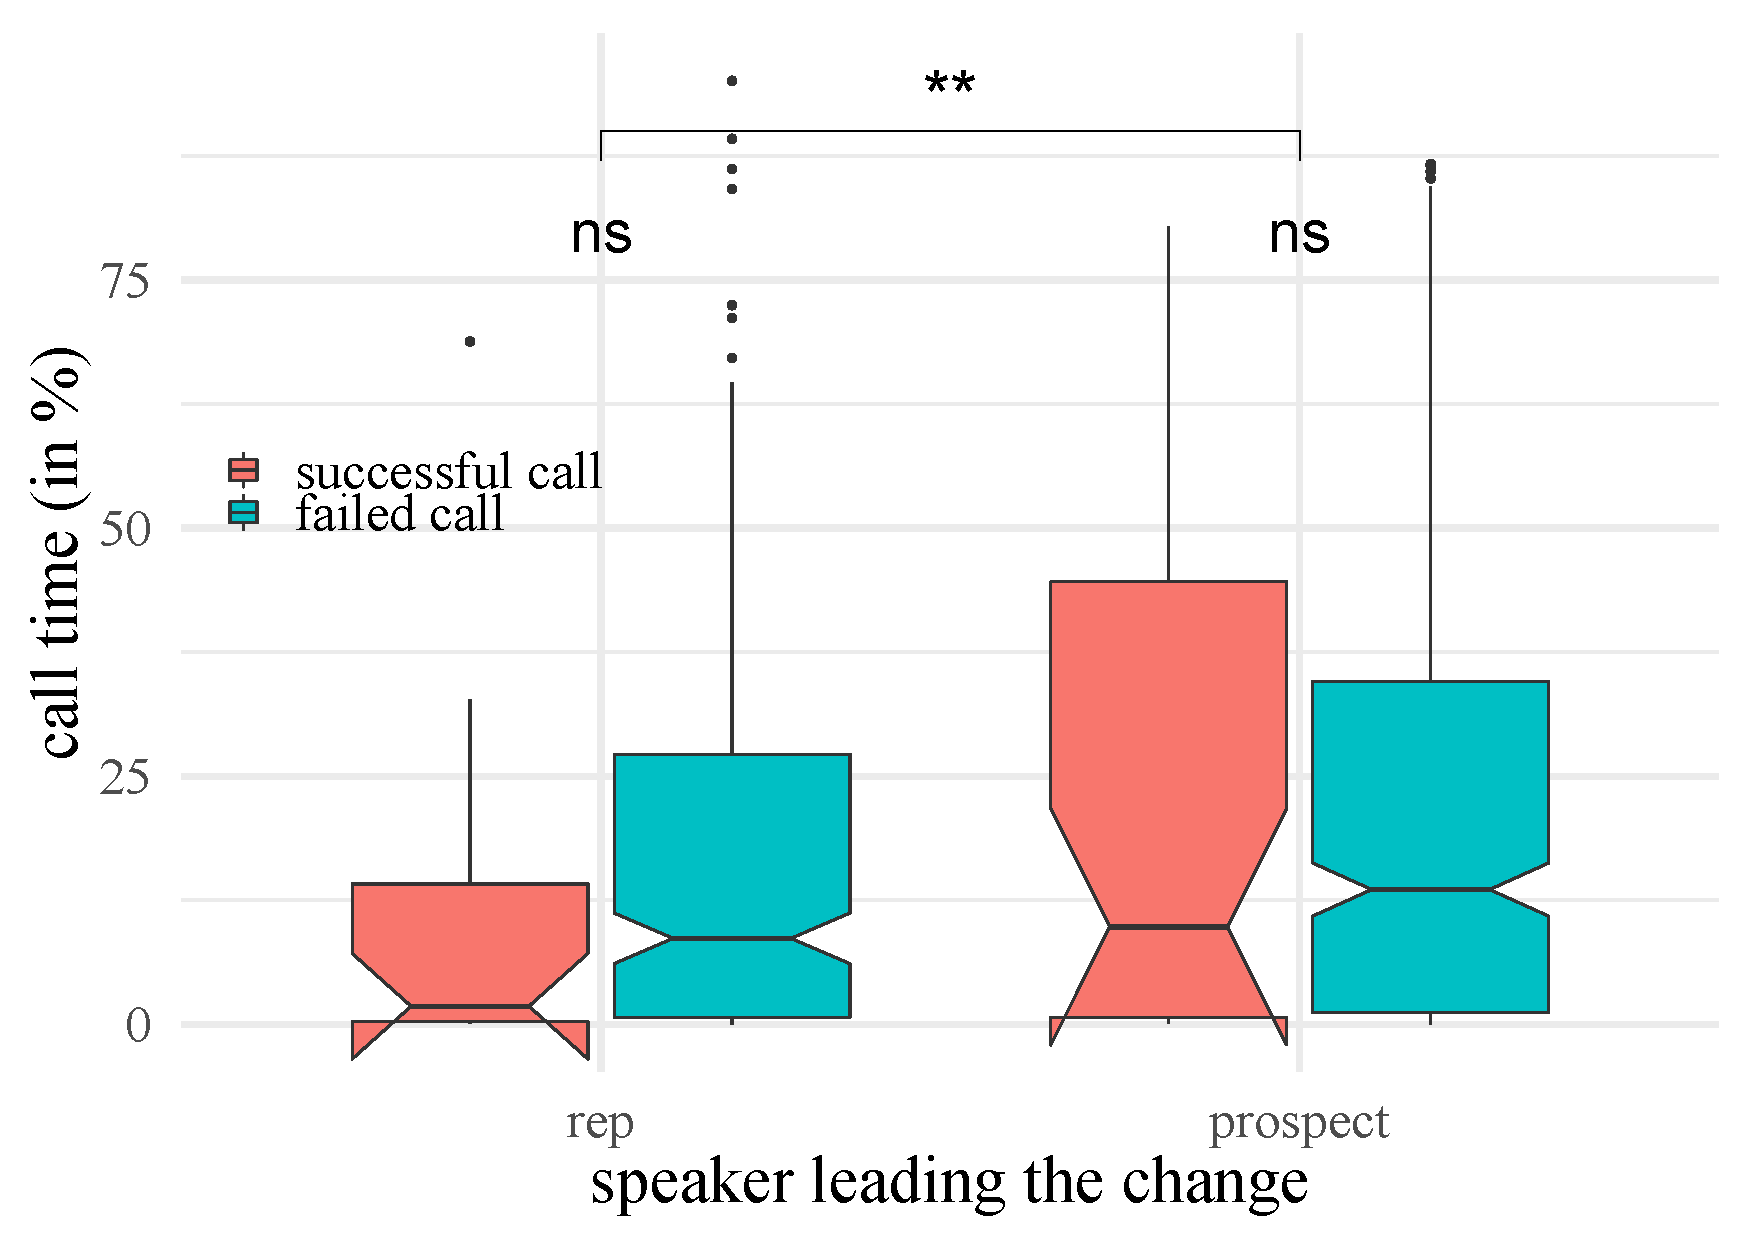
\includegraphics[width=\linewidth]{boxplot_ccf}
	\caption[Representatives' and prospects' lead-taking times in successful and failed calls]
		{Comparison between the time of the call in which the maximal cross-correlation occurs.
		The x-axis groups the calls based on the speaker role, and the fill color further separates between successful and failed calls.
		The y-axis shows the conversation timeline in percent (\SI{50}{\percent} marks the middle of the conversation).
		The horizontal lines in the boxes represent the median
		and he notches stand for the \SI{95}{\percent} confident level.
		% The area inside the boxes include the \acf{iqr} of values, the vertical lines outside the boxes show the value within the third quartile + 1.5$\protect\cdot$\ac{iqr}, and the isolated dots are the outliers.
		The significance level calculated with Wilcoxon test comparing the two groups and their subgroups is given above the boxes.}
	\label{fig:barplot_conv_leaders}
\end{figure}
%
Another known conversational element in sales calls is the floor time each speaker gets.
As a general approach, \acp{ae} aim to let the prospect talk as much as possible.
This is known to give them a better feeling during the call, and also give the reps more information and opportunities to understand what the customer wants to talk about.
Indeed, a recommended practice is to track the \emph{speech balance}, i.e., the ratio between the speaking time of the speakers.
Besides speech balance, the frequency and timing of floor switching also provide some insight on the dynamics of the speakers' vocal behaviors.
While each speaker should get a sufficient amount of time to talk, it is also important to take and give the floor to the other interlocutor when necessary.
Long monologues can make the listener lose concentration or lack of expression, which damages the interaction.
Therefore, the \emph{interactivity} of the speakers is important as well.
While speech balance informs about the overall amount of time each speaker talked, interactivity complements this by informing how often a speaker gave the floor to the conversation partner.
These two speech-related properties fit into the overall notion of vocal behavior.
Speech balance was measured by
%
\begin{equation}
	\label{eq:speech_balance}
	speech\_balance = 
	1 - \left| \frac{\displaystyle \sum_{\forall S \in S_A} dur(S) - 
						\sum_{\forall S \in S_B} dur(S)}
					{\displaystyle \sum_{\forall S \in S_A \cup S_B} dur(S)}
		\right|,
\end{equation}
\eqname{Speech balance in conversation}
\noindent
%
where $S_A$ and $S_B$ are the slices in which speakers $A$ and $B$ speak, respectively, and the function $dur$ returns the duration a slice.
The yielded value between 0 and 1 indicates the percentage of the balance in terms of speech times, with 1 standing for \enquote{perfect balance}, i.e., equal talking times for both speakers.
As mentioned above, the overall speech balance only reveals part of the whole picture.
Another part of it is the interactivity in the conversation, which is here defined as the percentage of slices in which floor change occurred after a sequence of longer than 1 slice was calculated.
Sequences below this threshold were treated as backchanneling, which does not indicate speaker change.
Interactivity and speech balance were measure for a superset of the dataset presented in \cref{sec:dataset_calls}.% which consisted of more than 1000 calls.
\cref{fig:speech-balance_success_violin} shows the speech balance scores of successful and failed calls.
On the one hand, it is clear that the lower the balance the more likely it was that reps had more floor time.
The recommendation to avoid imbalance is reflected by the significant difference between balance distribution in successful and failed calls.
On the other hand, prospects are only likely to talk more when the balance score is high, even more so in successful conversations.
This is accentuated by the highly significant differences in both sub-groups.
No significant influences of interactivity on call outcomes were found, and only a weak correlation between speech balance and interactivity was found ($\rho = 0.2$).
%
\begin{figure}
	\centering
	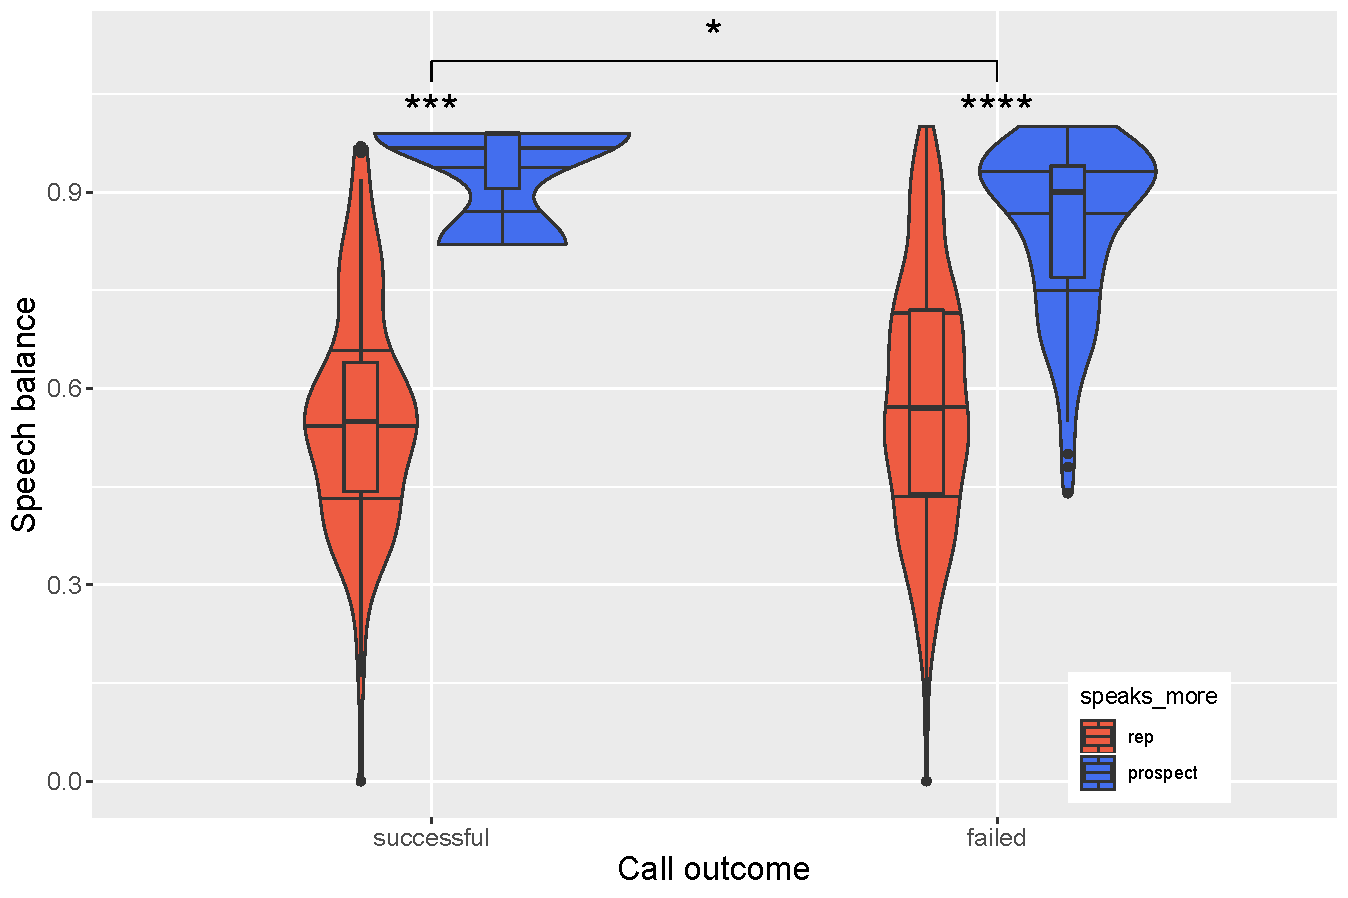
\includegraphics[width=\linewidth]{speech-balance_success_violin}
	\caption[Distribution of speech balance in successful and failed calls]
		{Comparison of speech balance distribution in successful and failed calls sub-grouped by the speaker who had more floor time in individual calls.
		The width of the shapes represent the probability density.
		The inner boxes show the central quartiles of the data.
		The medians are marked by the thick horizontal lines in the boxes.
		The additional horizontal lines mark the \SI{25}{\percent}, \SI{50}{\percent}, and \SI{75}{\percent} quartiles of the data.
		The asterisks above the shapes denote the significance levels of the comparisons between the main groups (successful vs.\ failed) and the subgroups (* $p < 0.05$, *** $p < 0.001$, **** $p < 0.0001$).}
	\label{fig:speech-balance_success_violin}
\end{figure}

\section{Conclusion}
\label{sec:conclusion_hhi}

The study presented in this chapter investigated accommodation occurrences in real-world sales conversations using \acf{crqa}.
Two main properties were examined, namely call success and role influence.
The results show that successful and failed calls significantly differed in three of the \ac{crqa} output values.
Although based on some \ac{hhi} studies it might be hypothesized that recurrence is more likely to occur in successful calls, the means of two of the three values suggest the opposite.
Yet, this stands in line with other studies from sales research that show more \enquote{desperate} behavior from the rep side when a deal is hard to close.
This includes unconsciously showing assimilation towards the prospect and over-emphasizing details, with the hope that it will convince the prospect to close a deal \citep{Orlob2018roi}.
However, these often achieve the opposite effect and are therefore discouraged in the sales industry.
Another possible explanation is that reps give up the lead when a call is on the verge of failing and instead let the prospects lead to give them a better feeling.
This, too, is a known effect in the sales business.
On the other hand, utilizing cross-correlation lags proved to be useful for differentiating between the leader in the calls.
When \acfp{ae} lead, they tend to do so at an earlier stage than prospects, especially in successful calls.

All these suggests that \acp{ae} do not necessarily always lead the conversation, but know how and when to exploit this technique, consciously or not, to improve their stance in calls.
It can be concluded that accommodation-related characteristics can be found in spontaneous, goal-oriented conversations and be used as a mean of analyzing their effectiveness.
However, despite anecdotal recommendations and recommended best practices, it cannot be claimed that exploitation of these effects \emph{directly influence} calls' success without further investigating, e.g., long-term performances of highly-rated reps.

%Though beyond the scope of this work, three further investigation directions on this topic are suggested here:
%First, deepening the aspect of the relationship between the \acp{ae} and the prospects by examining the mutual changes not only within single calls, but over the course of an entire deal spanning over several meetings.
%This could shed light on long-term changes and connect changes to the success of the deal.
%Secondly, distinguishing between different \acp{ae} to find behaviors of sub-groups or identifying star reps.
%For example, salespersons with higher ratings might be revealed to better exploit accommodation and trigger different behavior on the prospect side to increase their chance of closing a deal.
%Lastly, different methods could be applied to predict the success of a call.
%Specifically, machine learning methods that are good at capturing serial changes, such as recurrent neural networks, can be used to train such prediction models.
%All these directions can also be combined with more features to uncover more consistent accommodation patterns.

% Conclusion
%We have presented a study that examines phonetic accommodation in real-world sales calls.
%The focus was on mutual proximity of \acl{f0} between salespersons and prospects to find both how close they are to each other in general across the call, and how quickly changes in proximity occur and by whom they are initiated.
%This was done by \acf{crqa} and cross-correlations, which together provide various measures regarding recurrence between the speakers and who leads the other in terms of \acl{f0} changes.
%A corpus of 708 calls was used for the analyses, which makes it possible to find more global, consistent effects that are not influenced by the design of a specific experimental setting.
%The results show significant differences in some of the values between successful and failed calls, and significant differences between the leading behavior of salespersons and prospects.
%These findings encourage further investigations, like looking for other predictors of successful calls and examining the influence of additional features and factors on the success of calls.
